\documentclass[a4paper]{article}
\usepackage{graphicx}
\usepackage{onecolpceurws}
\usepackage[utf8]{inputenc}

\title{Granularity Social Network Analysis: Research in Progress}

\author{
Miguel Ángel Fernández \\ GSyC/LibreSoft \\
                Universidad Rey Juan Carlos \\ ma.fernandezsa@alumnos.urjc.es
\and
Gregorio Robles \\ GSyC/LibreSoft \\
                Universidad Rey Juan Carlos \\ grex@gsyc.urjc.es
\and
Jesús M. González Barahona \\ Bitergia \\
                jgb@bitergia.com
}

\institution{}


\begin{document}
\maketitle

\begin{abstract}
The Abstract paragraph should be indented $1.25$ inch on both
the left and right-hand margins. Abstract must be centered, bold, and
in point size 12. Two line spaces precede the Abstract. The Abstract
must be limited to one paragraph.
\end{abstract}
\vskip 32pt


\section{Introduction/Motivation}

Most social network studies for software projects are focused in a file-based
data of interactions in that network of developers. If there is a
collaboration between two or more developers in same file, how can we be sure
when there are thousands of lines of code if that people did actually
collaborate? \\
We want to go to a deeper level: in this particular case, a method-based
analysis which allows us to know with more accuracy if there is a real
relationship between those developers.

\section{Methodology}

The program studies registered changes made in a given repository tracked by
Git. From that repository, it extracts log from a specified date range. Using
that data, the program iterates with each commit made, and does a checkout
with all of them to take the repository to the state the program was when each
commit was made. At each iteration, we use Ctags with each file to get
classified all changes made in each of those files.\\ Next, is to find matches
between the commits information and Ctags data (still for each checkout), so
we can tell if a method has been modified.\\
Once the program finishes all checkout iterations, it takes that data and
searches for coincidences when different developers have modified same file
and method and outputs that data into two CSV-format files, one for in-file
collaborations and the other one for in-method collaborations; which can be
used in programs like Gephi to watch a graph-type representation of the
network.

\subsection{This is a subsection}

Other details about Methodology

\section{Case study: GNOME Gedit}

We used the program to study the evolution of GNOME-text editor Gedit. 
(https://github.com/GNOME/gedit).\\
The considered date range goes from the very beginning of the project (At
least, from the moment when log starts), which is April 15, 1998 until April
15, 2015.

\subsection{Results}

\subsubsection{Numeric results}

Here: numerical data and tables.

\subsubsection{Graphic results}

Figure 1 shows the different graphs (In-file and In-method data) from
first-half of 2001.\\

\begin{figure}[ht]
\begin{center}
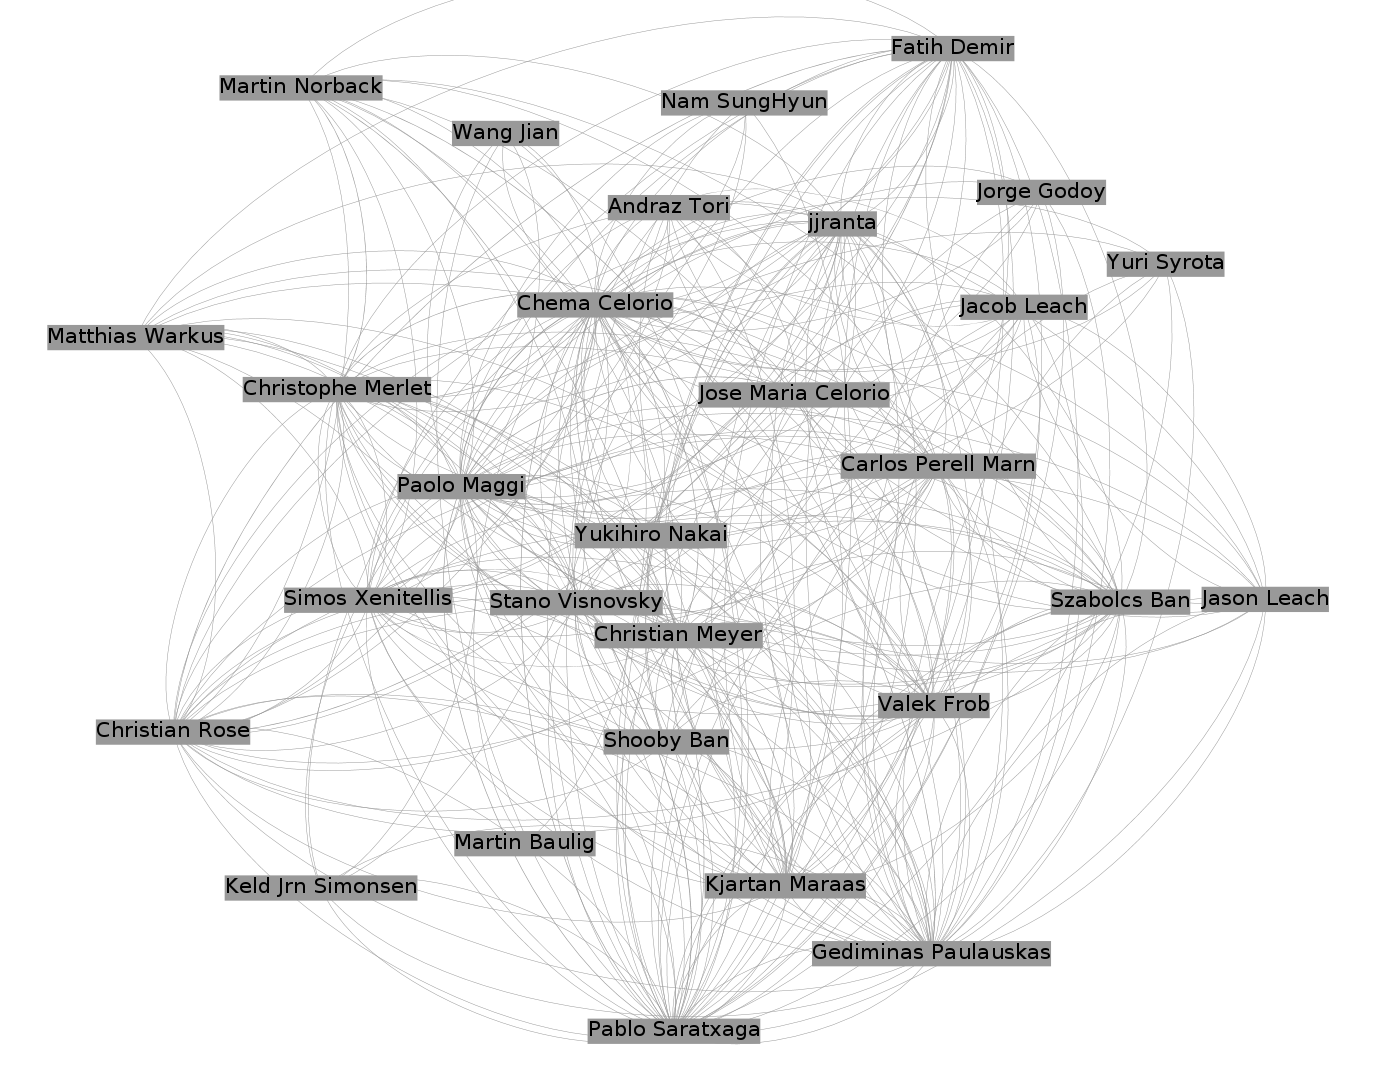
\includegraphics[scale=0.17]{g2001files.png} 
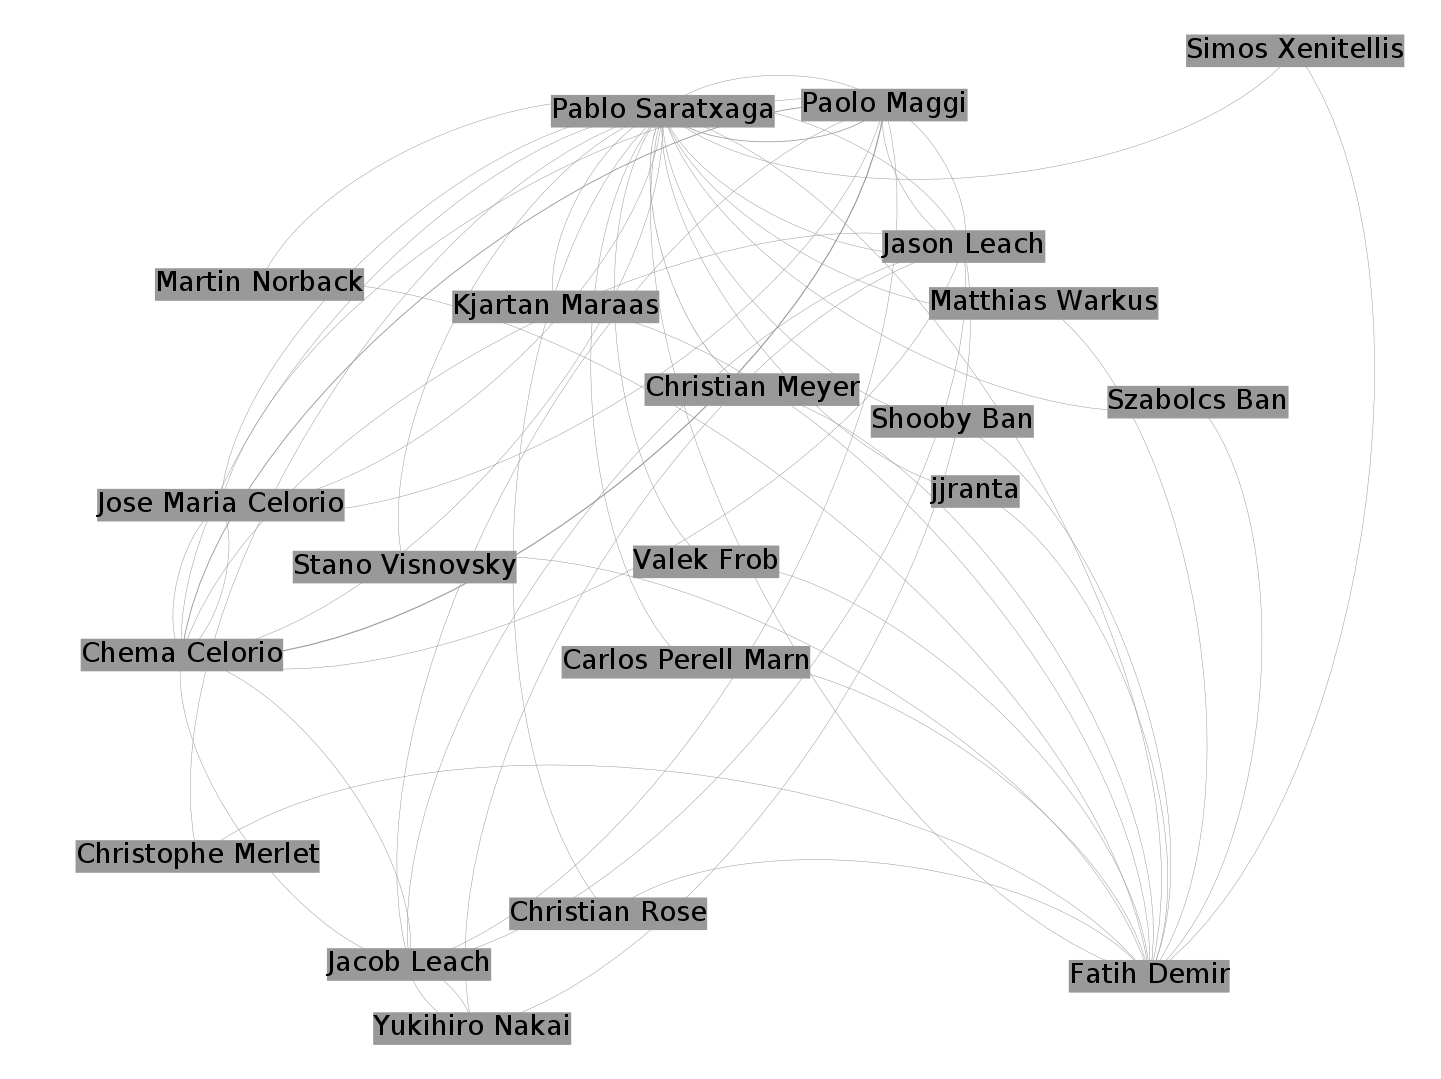
\includegraphics[scale=0.17]{g2001methods.png}
\caption{In-file (left) and In-method (right) collaboration graphs - 2001}
\label{fig1}
\end{center}
\end{figure}

\\
Figure 2 shows the different graphs (In-file and In-method data) from
second-half of 2014.\\

\begin{figure}[ht]
\begin{center}
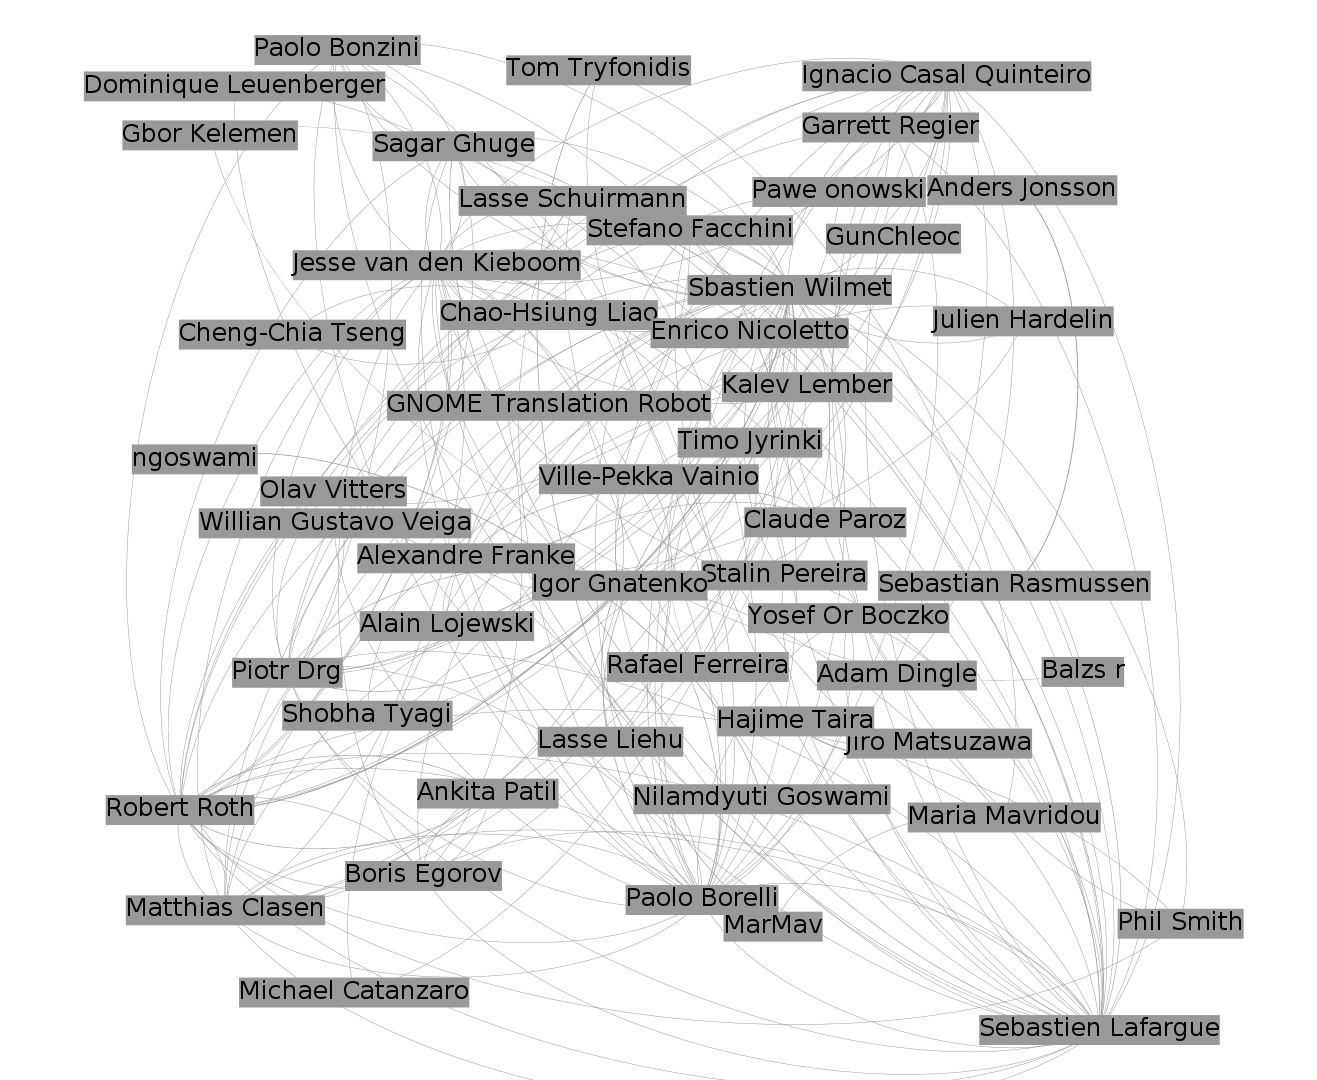
\includegraphics[scale=0.17]{g2014files.png} 
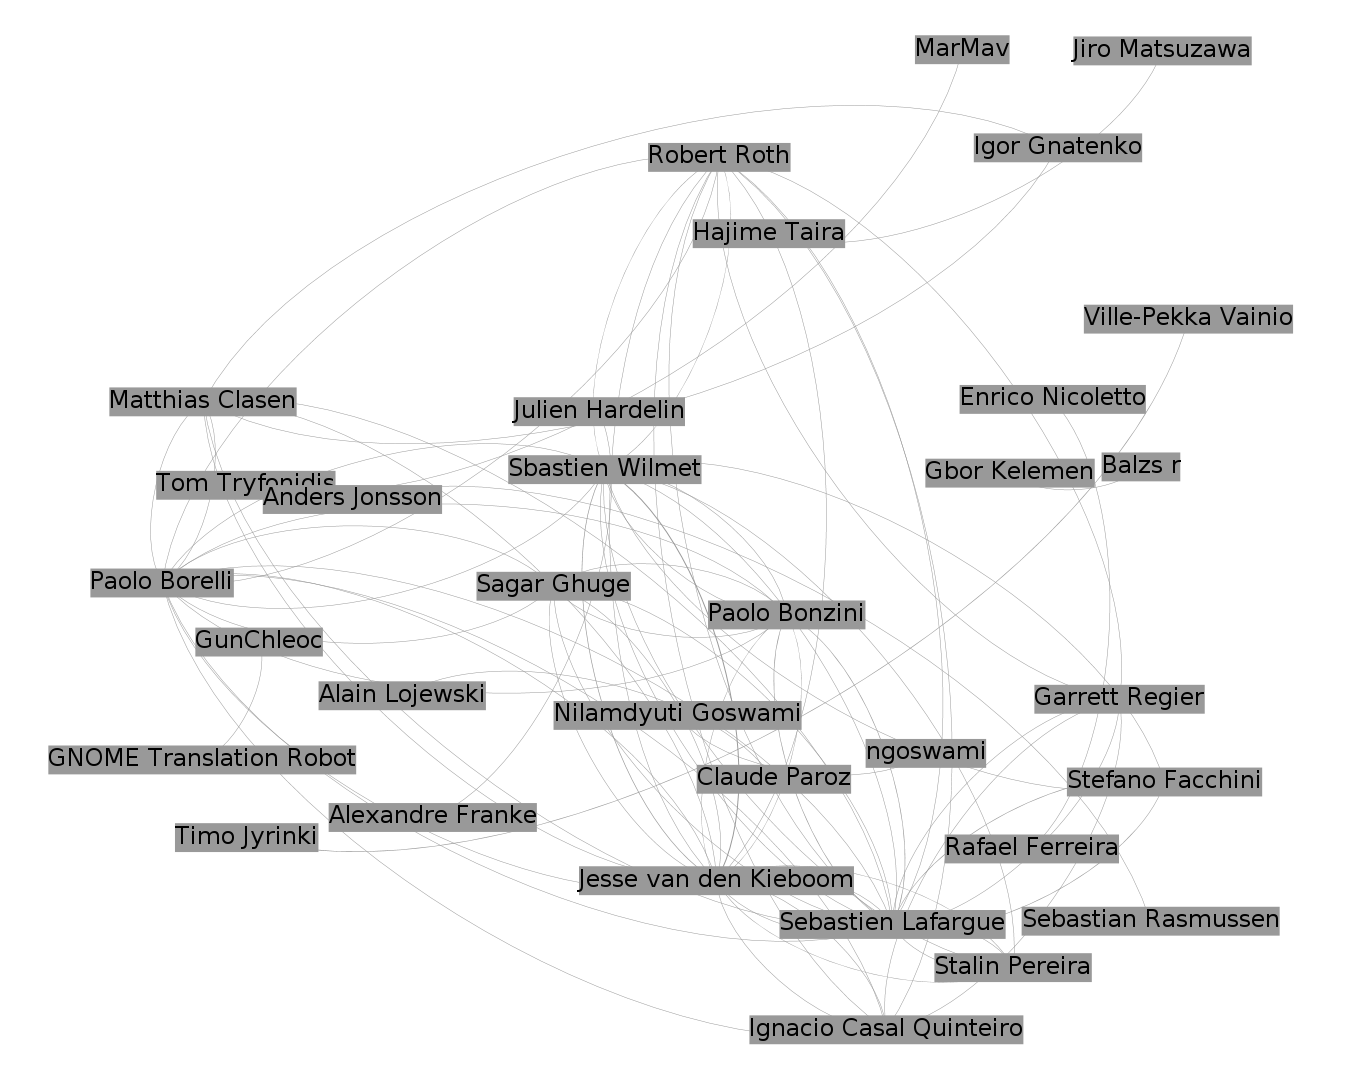
\includegraphics[scale=0.17]{g2014methods.png}
\caption{In-file (left) and In-method (right) collaboration graphs - 2014}
\label{fig1}
\end{center}
\end{figure}

Below is another figure using LaTeX commands.


\begin{figure}[ht]
\begin{center}
\setlength{\unitlength}{1pt}
\footnotesize
\begin{picture}(160,80)
        \put(0,0){\framebox(160,80)[]{}}
        \put(10,35){\framebox(80,40){}}
        \put(100,20){\framebox(40,20){}}
        \put(70,10){\framebox(20,10){}}
        \put(20,5){\framebox(10,5){}}
\end{picture}
\caption{Sample Figure Caption}
\end{center}
\end{figure}

\subsubsection{Tables}

All tables must be centred, neat, clean and legible. Do not use pencil
or hand-drawn tables. Table number and title always appear before the
table.

One line space before the table title, one line space after the table
title and one line space after the table. The table title must be
initial caps and each table numbered consecutively.

\begin{table}[ht]
\begin{center}
\caption{Sample Table}

\bigskip

\begin{tabular}{|l|l|r|}
\hline
A & B & 1\\ \hline
C & D & 2\\
E & F & 3\\ \hline
\end{tabular}
\end{center}
\end{table}


\subsubsection{Handling References}

Use a first level heading for the references. References follow the
acknowledgements.


\subsubsection{Acknowledgements}

Use a third level heading for the acknowledgements. All acknowledgements
go at the end of the paper.


\bibliographystyle{alpha} 
\bibliography{bib}
%inline the .bbl file directly for mailing to authors.

%\begin{thebibliography}{Com79}
%
%\bibitem[Com79]{Comer-btree}
%D.~Comer.
%\newblock The ubiquitous b-tree.
%\newblock {\em Computing Surveys}, 11(2):121--137, June 1979.
%
%\bibitem[Knu73]{Knuth-vol3}
%D.~E. Knuth.
%\newblock {\em The Art of Computer Programming -- Volume 3 / Sorting and
%  Searching}.
%\newblock Addison-Wesley, 1973.
%
%\end{thebibliography}

\end{document}


